\documentclass[a4paper]{article}

% Packages
\usepackage[utf8]{inputenc}
\usepackage{geometry}
\geometry{left=1.5cm, right=1.5cm, top=2.54cm, bottom=2.54cm}
\usepackage{graphicx, setspace, amsmath, amssymb, titlesec, fancyhdr, parskip, indentfirst, etoolbox, caption, cite, xcolor}
\usepackage{listings}
\usepackage{url}
\usepackage{hyperref}
\usepackage{multicol}
\usepackage{float} % PACOTE ADICIONADO AQUI
\usepackage[brazil]{babel}

\addto\captionsbrazil{
  \renewcommand{\refname}{Referências}
}

% Title Formatting
\titleformat{\section}{\centering\large\scshape}{\thesection}{1em}{}
\titleformat{\subsection}{\normalsize\bfseries}{\thesubsection.}{1em}{}

\setstretch{1.0}
\setlength{\parskip}{6pt}

\titlespacing{\section}{0pt}{6pt}{6pt}
\titlespacing{\subsection}{0pt}{6pt}{6pt}
\titlespacing{\subsubsection}{0pt}{6pt}{6pt}

% Document Title
\title{
    \textbf{Grupo 7 - Exercício 2}
}

\date{}

\captionsetup{labelfont={small,sc}, textfont={small,sc}}

% Section Numbering
\renewcommand{\thesection}{\Roman{section}.}
\renewcommand{\thesubsection}{\textit{\Alph{subsection}.}}
\renewcommand{\thesubsubsection}{\textit{\arabic{subsubsection}.}}
\renewcommand{\thetable}{\Roman{table}}
\renewcommand{\thefigure}{\Roman{figure}}

% Make titles italic as well
\titleformat{\subsection}
    {\normalfont\large\itshape}
    {\thesubsection}
    {1em}
    {}

\titleformat{\subsubsection}
    {\normalfont\itshape}
    {\thesubsubsection}
    {1em}
    {}

\setcounter{page}{1}

% Fancy Header Configuration
\pagestyle{fancy}
\fancyhf{}

% First Page Header
\fancypagestyle{firstpage}{
    \fancyhead[C]{
        \centering
        {\fontsize{14pt}{10pt}\selectfont
        \textbf{Universidade de São Paulo}\\[0.5em]
        \textbf{ACH2027 - Gestão de Projetos de Tecnologia da Informação}}\\[0.2em]
        {\fontsize{8pt}{10pt}\selectfont
        \textbf{Prof. Doutor:} Edmir Parada Vasques Prado \hspace{1cm}
        \textbf{Ano:} 2° Semestre/2026}
    }
}

% Default Header for Other Pages
\fancyhead[C]{
    \textbf{Escola de Artes, Ciências e Humanidades - Universidade de São Paulo}
}

\begin{document}

\maketitle
\vspace{-1.5cm}
\thispagestyle{firstpage}

% =========================================================
% INTEGRANTES
% =========================================================

\begin{multicols}{2}
    \centering

    \textbf{Gustavo G. França do Nascimento}\\
    15637551\\
    T94
    
    \vspace{0.5cm}
    
    \textbf{Kauã Lima de Souza}\\
    15674702\\
    T94
    
    \vspace{0.5cm}

    \textbf{Kevin Rodrigues Nunes}\\
    15676030\\
    T94
    
    \vspace{0.5cm}
    
    \textbf{Victor Yodono}\\
    13829040\\
    T94

\end{multicols}

\vspace{-0.2cm} % Ajuste de espaçamento vertical

% =========================================================
% CONTEÚDO
% =========================================================

\singlespacing
\setlength{\parskip}{6pt}
\setlength{\parindent}{0.5cm}

\section{Atividades da Estrutura Analítica do Projeto (EAP)}

A Estrutura Analítica do Projeto (EAP) apresenta a decomposição hierárquica do trabalho necessário para atingir os objetivos do projeto. O diagrama a seguir ilustra as principais fases e entregas.

% AJUSTADO PARA [H]
\begin{figure}[H]
    \centering
    % Substitua o nome do arquivo pela imagem da sua EAP ou WBS gerado
    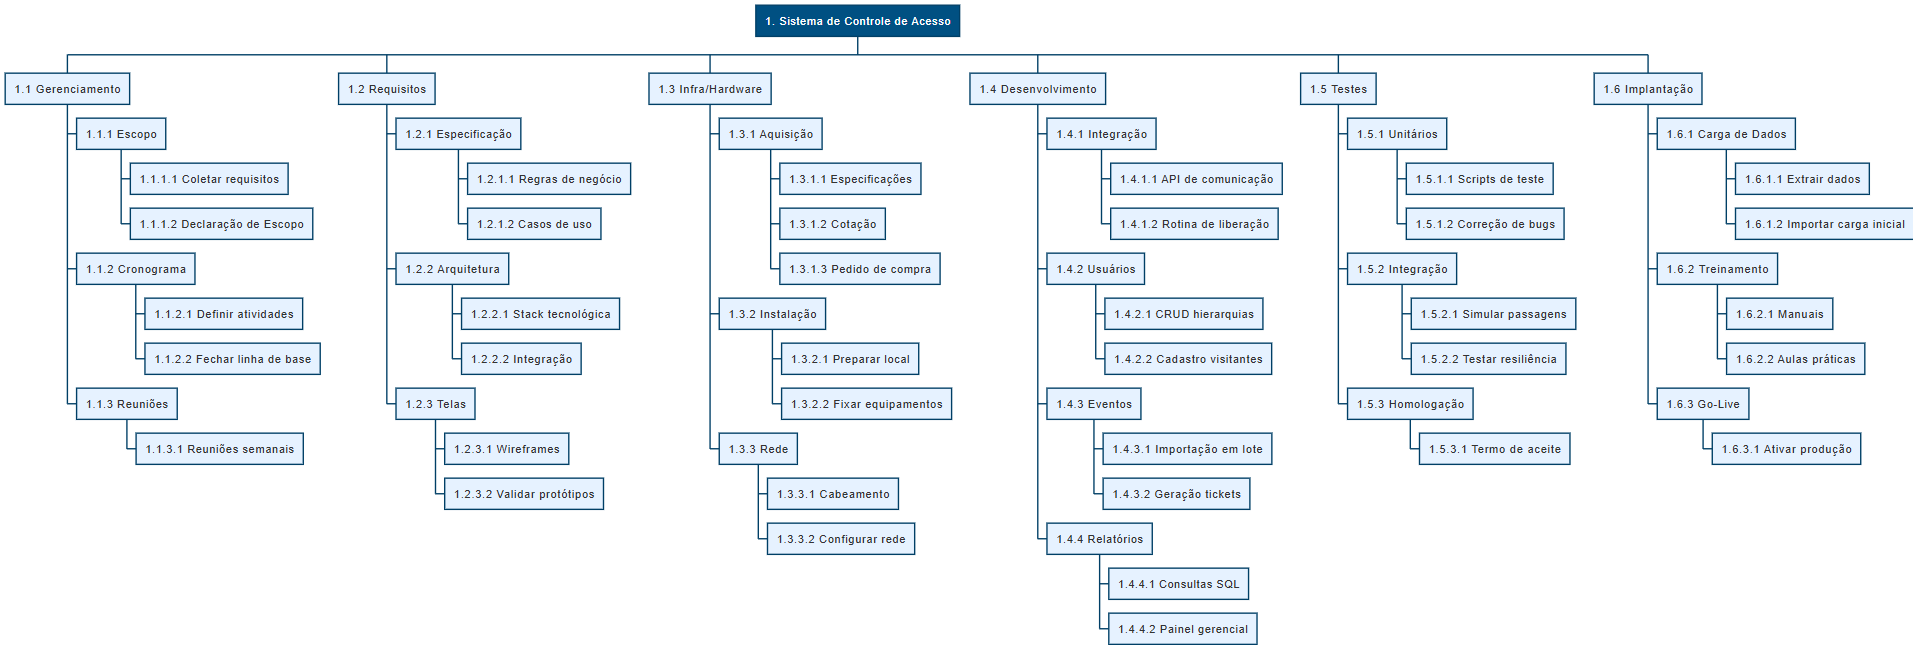
\includegraphics[width=\textwidth, height=0.85\textheight, keepaspectratio]{abcd.png}
    \caption{Estrutura Analítica do Projeto (EAP)}
    \label{fig:eap}
\end{figure}

\section{Duração das Atividades}

Em alinhamento aos processos de gerenciamento de tempo do PMBOK, os pacotes de trabalho oriundos da Estrutura Analítica do Projeto (EAP) foram decompostos em atividades menores e gerenciáveis. Abaixo, apresentamos a tabela consolidada com as estimativas de duração, seguida pelo detalhamento das relações lógicas de precedência para a construção do cronograma.

% AJUSTADO PARA [H]
\begin{table}[H]
    \centering
    \renewcommand{\arraystretch}{1.2}
    \small
    \begin{tabular}{|l|p{8cm}|c|}
        \hline
        \textbf{ID} & \textbf{Atividade} & \textbf{Duração} \\
        \hline
        1.1.1.1 & Coletar requisitos & 1 sem \\
        \hline
        1.1.1.2 & Declaração de Escopo & 1 sem \\
        \hline
        1.1.2.1 & Definir atividades & 1 sem \\
        \hline
        1.1.2.2 & Fechar linha de base & 1 sem \\
        \hline
        1.1.3.1 & Reuniões semanais & 24 sem \\
        \hline
        1.2.1.1 & Regras de negócio & 1 sem \\
        \hline
        1.2.1.2 & Casos de uso & 2 sem \\
        \hline
        1.2.2.1 & Stack tecnológica & 1 sem \\
        \hline
        1.2.2.2 & Integração & 2 sem \\
        \hline
        1.2.3.1 & Prototipar Wireframes & 1 sem \\
        \hline
        1.2.3.2 & Validar protótipos & 1 sem \\
        \hline
        1.3.1.1 & Especificações & 1 sem \\
        \hline
        1.3.1.2 & Cotação & 2 sem \\
        \hline
        1.3.1.3 & Pedido de compra & 4 sem \\
        \hline
        1.3.2.1 & Preparar local & 1 sem \\
        \hline
        1.3.2.2 & Fixar equipamentos & 2 sem \\
        \hline
        1.3.3.1 & Cabeamento & 1 sem \\
        \hline
        1.3.3.2 & Configurar rede & 1 sem \\
        \hline
        1.4.1.1 & API de comunicação & 3 sem \\
        \hline
        1.4.1.2 & Rotina de liberação & 2 sem \\
        \hline
        1.4.2.1 & CRUD hierarquias & 3 sem \\
        \hline
        1.4.2.2 & Cadastro visitantes & 2 sem \\
        \hline
        1.4.3.1 & Importação em lote & 2 sem \\
        \hline
        1.4.3.2 & Geração tickets & 1 sem \\
        \hline
        1.4.4.1 & Consultas SQL & 1 sem \\
        \hline
        1.4.4.2 & Painel gerencial & 2 sem \\
        \hline
        1.5.1.1 & Scripts de teste & 2 sem \\
        \hline
        1.5.1.2 & Correção de bugs & 1 sem \\
        \hline
        1.5.2.1 & Simular passagens & 1 sem \\
        \hline
        1.5.2.2 & Testar resiliência & 1 sem \\
        \hline
        1.5.3.1 & Termo de aceite & 1 sem \\
        \hline
        1.6.1.1 & Extrair dados & 1 sem \\
        \hline
        1.6.1.2 & Importar carga inicial & 1 sem \\
        \hline
        1.6.2.1 & Manuais & 1 sem \\
        \hline
        1.6.2.2 & Aulas práticas & 1 sem \\
        \hline
        1.6.3.1 & Ativar produção & 1 sem \\
        \hline
    \end{tabular}
    \caption{Esboço da estimativa de duração das atividades do projeto.}
    \label{tab:duracao_atividades}
\end{table}

\section{Registro de Uso de Inteligência Artificial}

Em conformidade com a Política de Uso de Ferramentas de Inteligência Artificial Generativa da disciplina ACH2027, declaramos explicitamente a utilização de IA como suporte ao aprendizado, ideação e estruturação deste documento. O quadro a seguir detalha os comandos utilizados, a ferramenta e a avaliação crítica dos resultados.

\begin{table}[H]
    \centering
    \renewcommand{\arraystretch}{1.5}
    \small 
    \begin{tabular}{|p{4cm}|p{11cm}|}
        \hline
        \textbf{Registro de Uso de IA} & \textbf{Registro 01: Diagramação da EAP} \\
        \hline
        \textbf{Problema / Objetivo} & Criar o diagrama visual da Estrutura Analítica do Projeto (EAP) e fazer um esboço da duração das atividades. \\
        \hline
        \textbf{Ferramenta de IA} & Gemini (Setembro/2026). \\
        \hline
        \textbf{Comandos} & "faça um esboço da estrutura analítica... precisa ser um diagrama" \\
        \hline
        \textbf{Revisão dos resultados} & Analisamos que o esboço da duração foi feito a partir do esboço do EAP original, que estava simplificado e não possuía todas as atividades. Pedimos para gerar as atividades e recalcular. Além disso, foi gerado de forma muito detalhada, incluindo reuniões diárias no EAP e estimando em 24 semanas. O grupo decidiu remover isso na próxima entrega. \\
        \hline
        \textbf{Aplicação no trabalho} & Seção da Estrutura Analítica do Projeto (EAP). \\
        \hline
    \end{tabular}
    \caption{Registro de Uso de IA Generativa.}
    \label{tab:uso_ia}
\end{table}

\begin{thebibliography}{99}

\bibitem{pmi2021}
PMI - PROJECT MANAGEMENT INSTITUTE. \textbf{Um Guia do Conhecimento em Gerenciamento de Projetos (Guia PMBOK)}. 7. ed. Pensilvânia: Project Management Institute, 2021.

\end{thebibliography}

\end{document}